\section{Quantization: Uniform}
\label{sec:Quantization: Uniform}

Computing the Signal to quantization Noise ratio of Uniform Quantization. 
Plot SNQR vs. Quantization levels.

\subsection{Matlab Code}

\inputminted[fontsize=\footnotesize,autogobble]{matlab}{code/sqnr.m}

\pagebreak

\subsection{Output}

\begin{figure}[!htb]
	\centering
	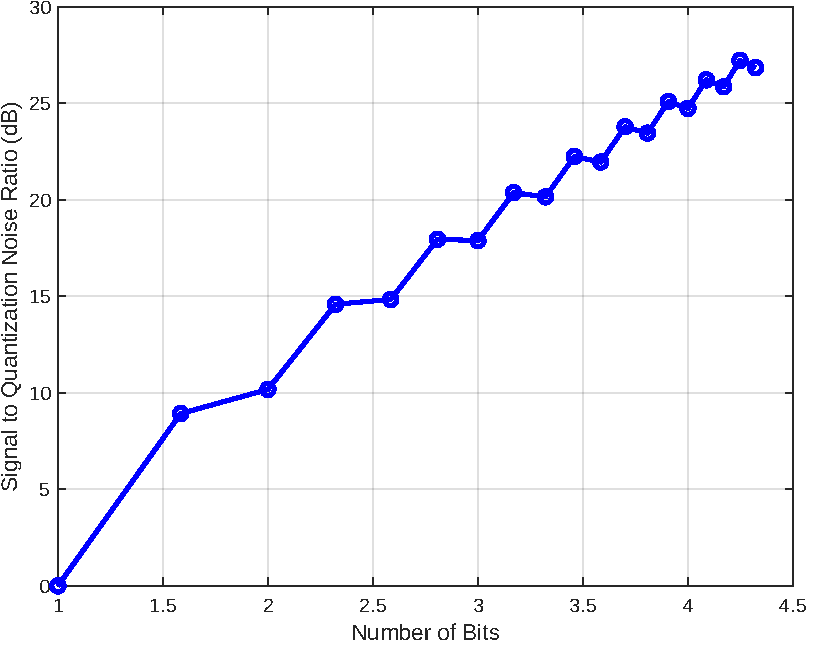
\includegraphics[width=6in]{res/figures/Figure_3.pdf}
	\label{output:SQNR vs quantization}
	\caption{SQNR vs Quantization}
\end{figure}

\section{Quantization: Non-Uniform}
\label{sec:Quantization: Non-Uniform}

Computing SNR of Non-Uniform Quantization and Plot SNR vs. Quantization Levels

\subsection{Matlab Code}

\inputminted[fontsize=\footnotesize,autogobble]{matlab}{code/sqnr2.m}
\subsection{Output}

\begin{figure}[!htb]
	\centering
	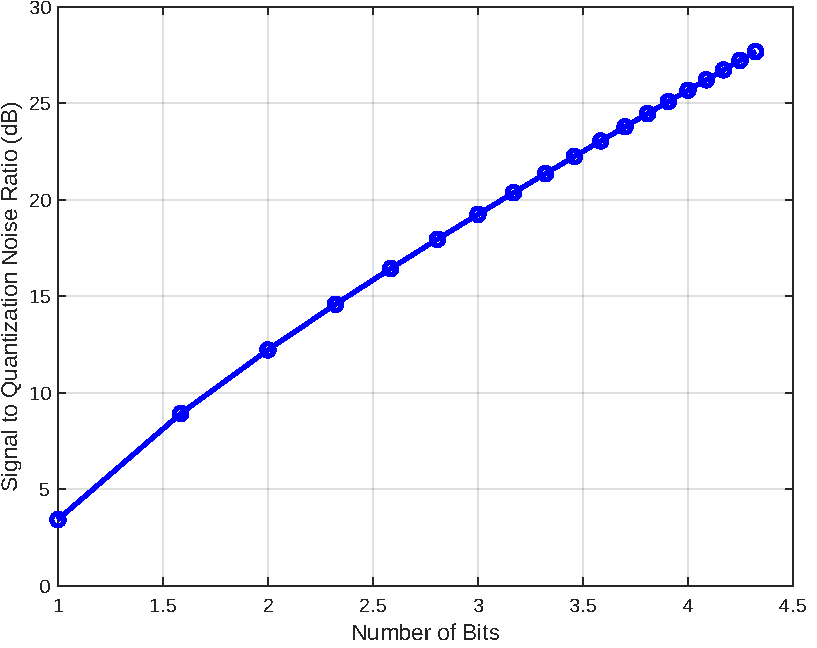
\includegraphics[width=5in]{res/figures/Figure_4.pdf}
	\label{output:SQNR vs quantization 2}
	\caption{SQNR vs Quantization (non-uniform)}
\end{figure}